\documentclass[tikz,border=2pt]{standalone}
\usepackage{amsmath}
\usepackage{pgfplots}
\pgfplotsset{compat=1.18}
\usetikzlibrary{arrows.meta}
\begin{document}
% x_{t+1} = -0.8 x_t + 9 from x_0 = 0: x_t = 5 + (-0.8)^t (x_0 - 5) = 0, 9, 1.8, ... alternates around
% x* = 5 inside the shrinking envelope 5 +- 5(0.8)^t, because |a| = 0.8 < 1.
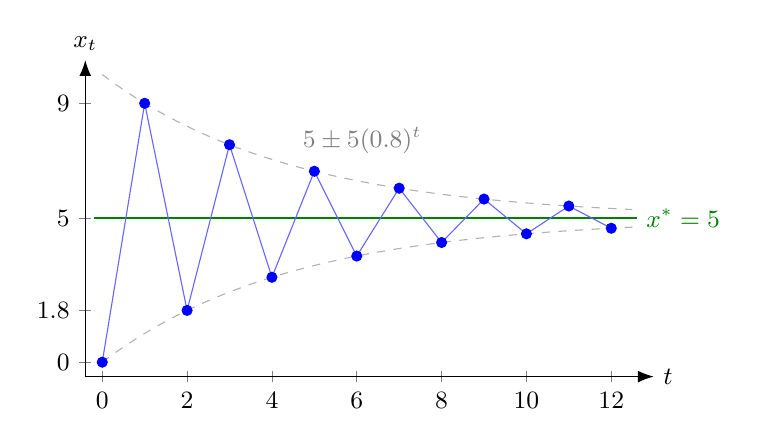
\begin{tikzpicture}[font=\small, >={Latex[length=2mm]}]
  \begin{axis}[width=8.8cm, height=5.6cm, axis lines=left, axis line style={->},
      xmin=-0.4, xmax=13, ymin=-0.5, ymax=10.5, xtick={0,2,4,6,8,10,12}, ytick={0,1.8,5,9},
      yticklabels={$0$,$1.8$,$5$,$9$},
      xlabel={$t$}, ylabel={$x_t$}, xlabel style={at={(1,0)}, anchor=west},
      ylabel style={at={(0,1)}, anchor=south, rotate=-90},
      tick label style={font=\small}, clip=false]
    \addplot[gray!60, dashed, domain=0:12.5, samples=80] {5+5*0.8^x};
    \addplot[gray!60, dashed, domain=0:12.5, samples=80] {5-5*0.8^x};
    \addplot[green!50!black, thick, domain=-0.2:12.6] {5};
    \addplot[blue!60, thin] coordinates {(0,0.0000) (1,9.0000) (2,1.8000) (3,7.5600) (4,2.9520) (5,6.6384) (6,3.6893) (7,6.0486) (8,4.1611) (9,5.6711) (10,4.4631) (11,5.4295) (12,4.6564)};
    \addplot[only marks, mark=*, mark size=1.8pt, blue] coordinates {(0,0.0000) (1,9.0000) (2,1.8000) (3,7.5600) (4,2.9520) (5,6.6384) (6,3.6893) (7,6.0486) (8,4.1611) (9,5.6711) (10,4.4631) (11,5.4295) (12,4.6564)};
    \node[green!50!black, anchor=west] at (axis cs:12.6,5) {$x^*=5$};
    \node[gray, anchor=south west] at (axis cs:4.5,6.9) {$5\pm5(0.8)^t$};
  \end{axis}
\end{tikzpicture}
\end{document}
